\documentclass{article}
\usepackage[english]{babel}
\usepackage[utf8]{inputenc}
\usepackage{fancyhdr}
\usepackage{amsmath}
\usepackage{pdfpages}

\pagestyle{fancy}
\fancyhf{}
\rhead{CS760}
\lhead{Cheng-Wei Lu}
\rfoot{Page \thepage}

\begin{document}

\section*{CS 760 Homework 4 by Cheng-Wei Lu}

\subsection*{Problem 4.1}
	For each non-binary feature, I use its average as a standard to decide the binary transformation of each data. I use average because in reality, we often divide data in two parts with average. Therefore, I think it would also be reasonable if I use average here. If the original feature is greater than the average, it will be converted to 1. If not, it will be converted to 0. The average for passenger class is 2.3, age is 29.4, siblings/spouses aboard is 0.5, parents/children aboard is 0.4 and fare is 32.3.
\subsection*{Problem 4.2}
	Please see the appendix notebook cell of title, "Calculate mutual information (Problem 4.2)."

\subsection*{Problem 4.3}
	Please see the appendix notebook cell of title, "Build Decision Tree (Problem 4.3)."
	I stop the tree from growing more nodes when the entropy of y is less than 0.2 or when all the  features are tested.
	
\subsection*{Problem 4.4}
	Please see the appendix notebook cell of title, "Tree Displayed (Problem 4.4)." There you can see the structure of my tree.
	
\subsection*{Problem 4.5}
	Please see the appendix notebook cell of title, "10 fold cross validation (Problem 4.5)." The accuracy of my prediction is 0.813.
	
\subsection*{Problem 4.6}
	My original data is 
	\begin{equation*}
	\begin{pmatrix} 2 \text{(class)}\\ 0 \text{(sex)}\\ 25\text{(age)}\\ 0\text{(siblings/spouses aboard)}\\0\text{(parents/children aboard)}\\ 50\text{(fare)}\end{pmatrix} 
	\end{equation*}.
	
	According to the conversion rule, my data input to the decision tree will be,
\begin{equation*}	
	\begin{pmatrix} 0 \text{(class)}\\ 0 \text{(sex)}\\ 0\text{(age)}\\ 0\text{(siblings/spouses aboard)}\\0\text{(parents/children aboard)}\\ 1\text{(fare)}\end{pmatrix} 
	\end{equation*}.
	
	According to my decision tree, I wouldn't have survived.
\subsection*{Problem 4.7}
\subsubsection*{(a)}
	Please see the appendix notebook cell of title, "Random Forest on Sampling - Trees Displayed (Problem 4.7(a))." There you can see the structure of my trees.
\subsubsection*{(b)}
	The accuracy is  0.831
\subsubsection*{(c)}
	According to my random forest, I wouldn't have survived.

\subsection*{Problem 4.8}
\subsubsection*{(a)}
	Please see the appendix notebook cell of title, " Random Forest on Feature Dropping - Trees Displayed (Problem 4.8(a))." There you can see the structure of my trees.
	
\subsubsection*{(b)}
	The accuracy is  0.825
	
\subsubsection*{(c)}
	According to my random forest, I wouldn't have survived.
	
\subsection*{Problem 4.9}
	Yes, my predictions all agree with each other. I would like to use logistic regression more, because with logistic regression, we analyze more detailedly on the relationship between the coefficient of a feature with the prediction result.
	
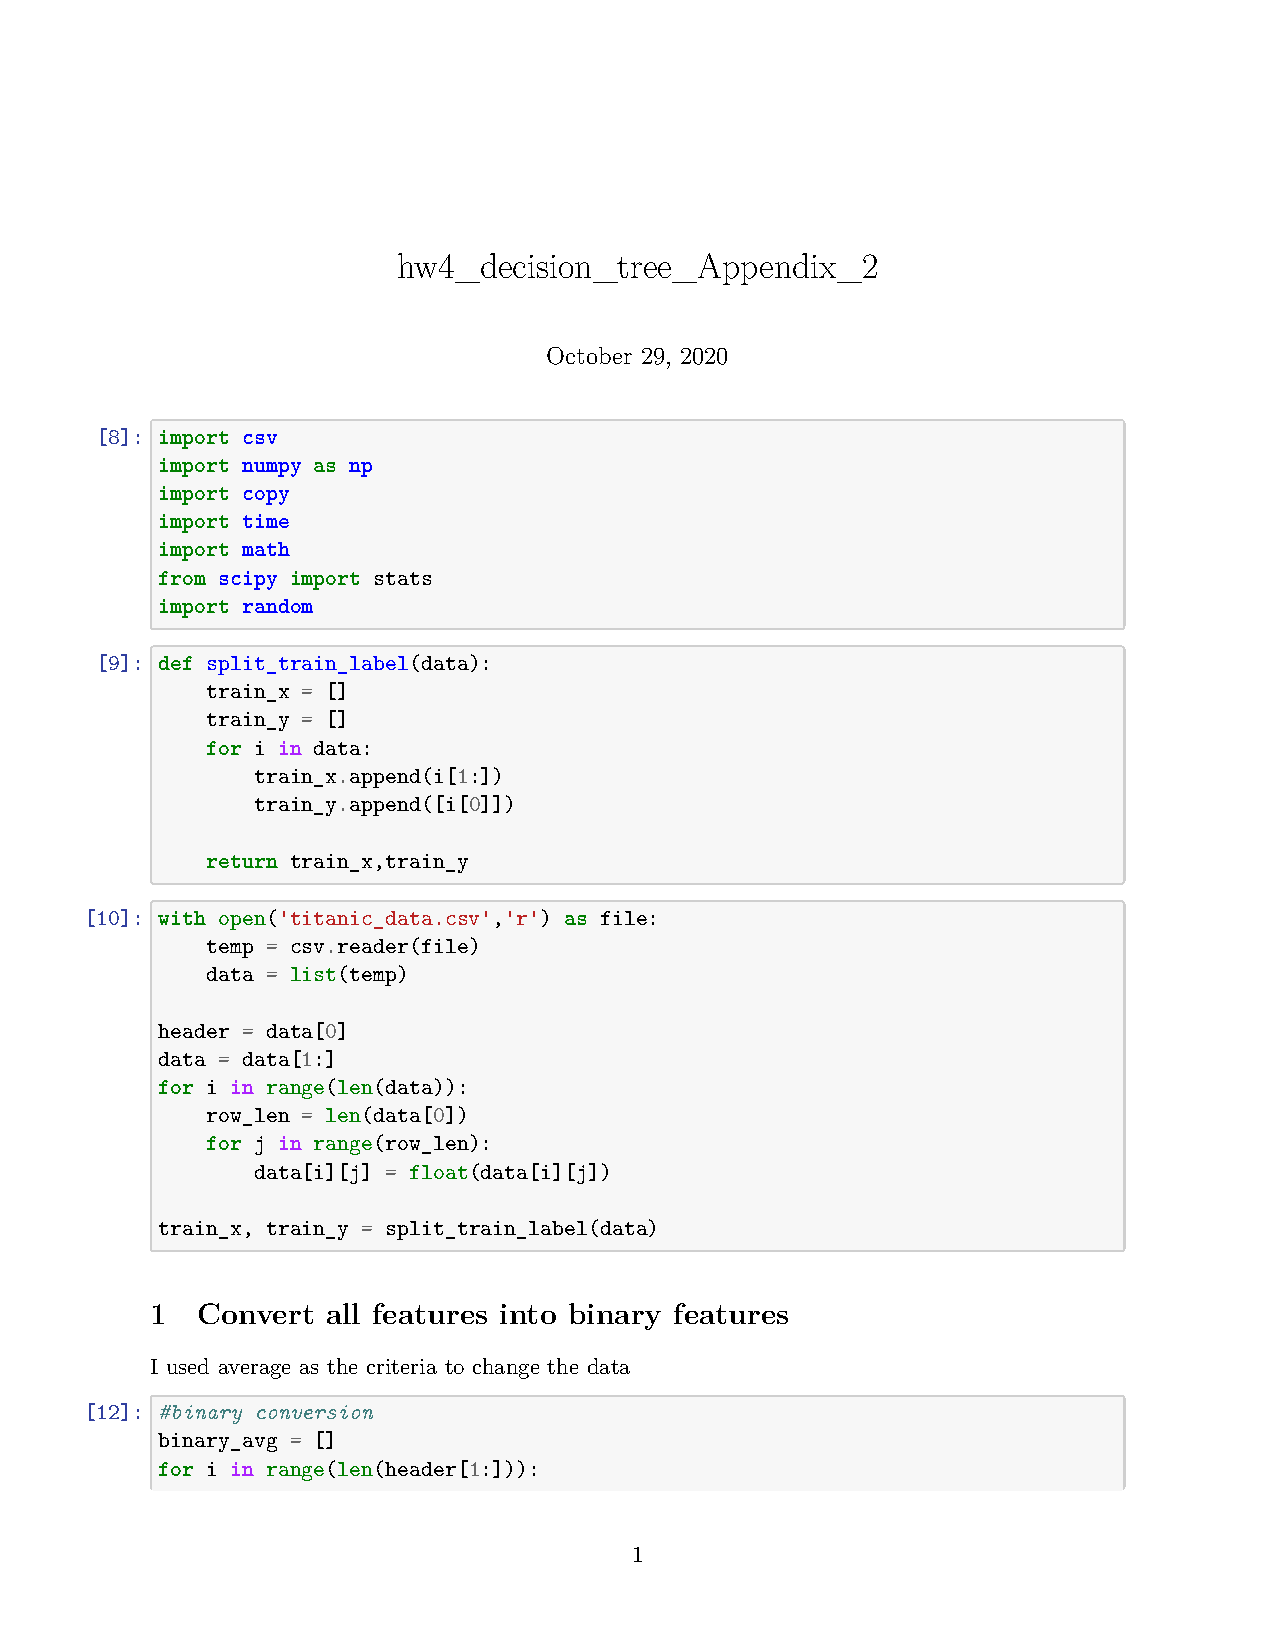
\includepdf[page={1-}]{hw4_decision_tree_Appendix_2.pdf}


\end{document}